\documentclass[12pt,a4paper,titlepage]{article}
%\documentclass[12pt, a4paper, UTF8]{ctexart}
\usepackage{CJK}

\usepackage{ctex}
\usepackage{lipsum}     %随机生成文本的宏包
\usepackage{geometry}   %设置页边距的宏包
\usepackage{titlesec}   %设置页眉页脚的宏包
\usepackage{setspace}   %行距
\usepackage{fancyhdr}	   %页眉页脚  
%\usepackage{titlesec}   %设置子标题字体
\usepackage{titlesec}
\usepackage[colorlinks,linkcolor=black]{hyperref}  %超链接
\usepackage{epsfig}           %插图
\usepackage{graphicx}
\usepackage{subfigure}
\usepackage{enumitem}
\usepackage{amsmath}          %split

%说明。bibtex如果需要引用中文文献,编码方式要一致,否则乱码,我的是使用utf-8无签名就不会乱码。

\setCJKmainfont{宋体}   %全局中文环境

\setenumerate[1]{itemsep=0pt,partopsep=0pt,parsep=\parskip,topsep=5pt}
\setitemize[1]{itemsep=0pt,partopsep=0pt,parsep=\parskip,topsep=5pt}
\setdescription{itemsep=0pt,partopsep=0pt,parsep=\parskip,topsep=5pt}

\titleformat{\paragraph}[block]{\normalsize\bfseries}{\theparagraph}{1em}{}  %paragraph 换行


\titleformat{\section}%设置section的样式
{\center\zihao{-2}\bfseries}%右对齐,小二号字,加粗
{\thesection .\quad}%标号后面有个点
{0pt}%sep label和title之间的水平距离
{}%标题前没有内容

\titleformat{\subsection}%设置section的样式
{\raggedright\zihao{-3}\bfseries}%右对齐,小三号字,加粗
{\thesubsection.\quad}%标号后面有个点
{0pt}%sep label和title之间的水平距离
{}%标题前没有内容

\titleformat{\subsubsection}%设置section的样式
{\raggedright\zihao{4}\bfseries}%右对齐,四号字,加粗
{\thesubsubsection.\quad}%标号后面有个点
{0pt}%sep label和title之间的水平距离
{}%标题前没有内容 

\newcommand{\upcite}[1]{\textsuperscript{\textsuperscript{\cite{#1}}}}  %引用右上角


\pagestyle{fancy}
\fancyhf{}
\setlength{\baselineskip}{18pt}
\geometry{left=3cm,right=2.5cm,top=2.5cm,bottom=2.5cm}  %设置 上、左、下、右 页边距



\cfoot{\zihao{5} \thepage}
\fancyhead[CO,CE]{\zihao{4} 安徽工业大学毕业设计}


\title{基于深度卷积神经网络和迁移学习的行人检测算法探究与实现}
\author{吴若晨}
\date{\today}




\begin{document}




\renewcommand{\figurename}{图}
\maketitle

\renewcommand{\abstractname}{\zihao{3} 摘要}
\begin{abstract}
\qquad 行人检测,是利用计算机视觉技术在静态图像或动态视频序列中,查找并定位行人的算法。由于其应用方向广,挑战难度大,所有学术工业界均有着深入的研究。
传统行人检测算法,如Hog+SVM法,主要使用如下流程:提取静态特征(边缘特征,统计特征等),滑动窗口分类行人,但传统算法仍有许多不足:对模糊图像识别效果差,不能准确定位,漏识别,错识别概率高。\par
自Alexnet于2012年在ImageNet竞赛大放异彩开始,深度学习开始受到人们的广泛关注。其中深度卷积神经网络,由于其强大的特征提取特性,在计算机视觉各个方面上,都对传统方法实现了超越。
另一方面,深度卷积网络对数据集要求非常高,很多算法都是在小数据集上没法训练出令人满意的结果,所以研究人员通常采用的是迁移学习中微调的技术,首先在大型数据集上(如ImageNet)进行预训练,之后在得到的网络模型上再使用自身数据集进行训练,这样往往能够保证效果。\par
本毕设的构想是通过复现基于深度卷积网络的几个物体检测算法,如Faster-RCNN,YOLO,SSD,利用微调技术,将它们迁移至行人检测任务上来,并期望相较迁移学习前的算法,行人检测部分性能有所提升。
\begin{center}
{\textbf{关键词}:卷积神经网络,物体检测,迁移学习,行人检测}
\end{center}
\end{abstract}

\renewcommand{\abstractname}{\zihao{3} Abstract}
\begin{abstract}
\qquad Pedestrian detection is an algorithm to find and locate pedestrians in static image or dynamic video sequences using computer vision technology.
Because of its wide application prospect and great challenge, both Academia and Industry have much research on it.
The traditional pedestrian detection algorithm, such as Hog+SVM method,mainly follows these two steps:
extracting static features (edge feature, statistical feature etc), using sliding window to classify pedestrians.Still there are a good many deficiencies of traditional algorithms.
They have problem with processing fuzzy pedestrain, fail to precisely localize, and have a high error of wrong detection.\par
Since 2012 when AlexNet yields unusually brilliant results in the ImageNet competition,people have been arousing great interests in deep learning.
Meanwhile deep convolutional nerual network has surpassed the traditional methods in many aspects of computer vision due to its excellent ability of extracting features.
On the other hand, convolutional neural networks require large amounts of data, algorithm usually fails to work when training in small scale dataset.
To deal with it, reasearchers generally use the method fine-tuning,which is one of the effective way of transform learning.
First pre-train their model in the large data set (such as ImageNet) , then use their own data set(much smaller) to train, this strategy often effects.\par
This graduation project aims at reimplementing several state-of-art object detection algorithm, such as Faster-RCNN, YOLO, SSD, and transforming them to the task of pedestrain detection using the technology of fine-tuning.
Besides compared to the original object detection algorithm, these transformed method should perform better in this specific detection of pedestrain.
\begin{center}
{\textbf{keywords}: CNN, object detection, tranform learning, pedestrain detection}
\end{center}
\end{abstract}

\renewcommand{\contentsname}{目录}
\tableofcontents
\newpage

\section{绪论}
\subsection{研究背景及意义}
\subsubsection{研究背景}
行人检测作为计算机视觉中的一个经典的主题,其在学术界和工业界一直有着广泛的研究和应用。现有的行人检测方法主要为一些非深度方法,这些方法进一步又可分为基于背景建模的方法和基于机器学习的方法。背景建模法通过建立背景模型,利用背景减分割出前景,进一步判断和提取其中的行人目标。这类方法的抗干扰能力不强,难以处理背景的动态变化以及摄像头运动下拍摄的动态场景。而机器学习的方法,则是从大量训练样本中提取特征来构建行人分类器或者检测器\upcite{邵松2014基于迁移学习的行人检测研究进展}。总的来说,这些机器学习方法还停留在特征工程结合分类器的层面上,首先使用一系列手工特征的组合,如Integral channel features\upcite{dollar2009integral},HoG\upcite{dalal2005histograms}以及它们的变体\upcite{felzenszwalb2010object,schwartz2009human},再将这些提取的特征送入诸如SVM\upcite{felzenszwalb2010object},随机森林\upcite{dollar2012crosstalk}等分类器进行训练与测试。相较于背景建模的方法,机器学习方法对动态场景有着更强的鲁棒性和更低的误检率。然而,由于受限于浅层特征的表达能力,传统基于机器学习的行人检测算法,往往泛化能力较差,如果适用的场景与训练数据集差异很大,则这些方法的性能会急剧下降,为了解决问题,需要重新采集和标注大量的数据样本,耗时耗力,且若场景再次切换,需要重复如上工作。关于如何解决这个问题,学术界也对相应的机器学习方法细节进行了研究\upcite{邵松2014基于迁移学习的行人检测研究进展}。另外机器学习工业界广为流传着这样一句话:“数据和特征决定了机器学习的上限,而模型和算法只是逼近这个上限而已”,挖掘更高层次的特征,成为解决检测问题一大重要方向。\par
另一个方面,深度学习曾作为神经网络被我们广为熟知,在20世纪80年代流行过一阵,取到了相对较小的成功。但由于其收敛原因缺乏理论证明,深层网络对算力要求高等缺陷,而渐渐被研究人员抛弃。现如今随着与日俱增的数据量和不断增强的计算力,我们拥有的计算资源可以运行更大的模型,深度学习的精确识别和预测能力也一直在提高。深度卷积网络作为深度学习的一个子集,具有强大的特征提取能力,而这一特性,恰好适合计算机视觉中各类图像任务。关于深度学习能力的一个粗略的经验法则是:监督深度学习算法在每类给定约5000个标注样本情况下一般将达到可接受的性能,当至少有1000万个标注样本的数据集用于训练时,它将达到或超过人类表现\upcite{Goodfellow-et-al-2016}。深度学习随着卷积网络AlexNet\upcite{krizhevsky2012imagenet}在ImageNet竞赛大放异彩而迅速崛起,随后卷积网络在图像识别\upcite{simonyan2014very,he2016deep},物体检测\upcite{ren15fasterrcnn,redmon2016you,liu2016ssd}等各个方向实现了对传统方法的超越。特定到行人检测的深度学习方法,也有相关的研究\upcite{sermanet2013pedestrian}。关于神经网络和卷积网络,可参考本毕业设计于附录部分的简单介绍。

本课设旨在从深度学习中卷积神经网络的角度切入,改善非深度方法中对模糊图像处理乏力,泛化能力不强的缺陷。并相较传统方法,达到更高的准确率,和更低的漏检,错检率。 
\subsubsection{研究意义}


\subsection{国内外论文综述}
\subsubsection{国内相关行人检测研究}
几篇论文
\subsubsection{国外相关行人检测研究}
几篇论文

\subsection{研究方法与内容}
\subsubsection{研究方法}
深度卷积网络,迁移学习
\subsubsection{研究内容}
具体算法

\section{算法}
\subsection{传统算法}
Hog+SVM
\subsection{faster-RCNN}
\subsubsection{算法原理}
region proposal + classifier
\subsubsection{实验表现}
PASCAL VOC 71.2 mAP   15FPS
\subsection{YOLO}
\subsubsection{算法原理}
YOLO(You only look once)\upcite{redmon2016you}
\subsubsection{实验表现}
PACAL VOC 63.0 mAP    45FPS
\subsection{SSD}
\subsubsection{算法原理}
SSD\upcite{liu2016ssd}
\subsubsection{实验表现}


\section{算法的实际场景应用}

\section*{致谢}
\addcontentsline{toc}{section}{致谢}


\newpage
\renewcommand\refname{\zihao{-2} 参考文献}
\addcontentsline{toc}{section}{参考文献}
\bibliographystyle{unsrt}     %按引用顺序
\bibliography{bio}

\newpage
\section*{附录}
\addcontentsline{toc}{section}{附录}


\setcounter{section}{1}
\subsection*{神经网络简介及其在计算机视觉上的应用}
\subsubsection*{神经网络简介}

常见的神经网络结构是如图\ref{fig:nn}所示的层级结构。
\begin{figure}[htbp]
\begin{minipage}[t]{0.35\linewidth}
\centering
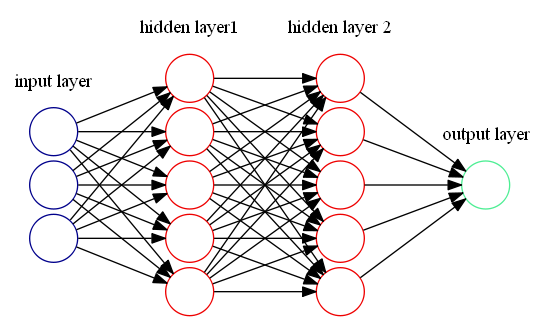
\includegraphics[height=4.5cm]{neural_network.png}
\caption{双隐层前馈网络}
\label{fig:nn}
\end{minipage}%
\hfill
\begin{minipage}[t]{0.5\linewidth}
\centering
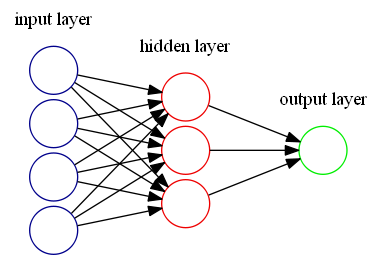
\includegraphics[height=4.5cm]{nn431.png}
\caption{4结点输入单隐藏层网络}
\label{fig:sample}
\end{minipage}
\end{figure}
图中,每个结点代表一个神经元,神经元是神经网络构成的最基本成分,当神经元的接收到的总输入值超过了阈值,则该神经元通过激活函数(activation function)对后续神经元产生输出。输入层与输出层之间的每层神经元,被称为隐层或者隐含层(hidden layer),隐含层和输出层的神经元都是拥有激活函数的功能神经元。每层神经元与下一层神经元全互联,神经元之间不存在同层连接,也不存在跨层连接。这样的神经网络结构通常称为“多层前馈神经网络”(multi-layer feedforward neural networks)。图示即为双隐层前馈网络。输入层神经元接受外界输入,隐层与输出层神经元对信号进行加工,最终结果由输出层神经元输出。神经网络的学习过程,就是根据训练数据来调整神经元之间的“连接权”(connection weight)以及每个功能神经元的阈值。\par
\subsubsection*{神经网络在计算机视觉上的应用}
以图像识别任务为例,假设一个图像是大小$2 \times 2$的灰度图像,那么在将它在计算机上将以一个$1 \times 2 \times 2$的矩阵储存,在送入神经网络进行分类之前,需要将其展开成一维向量。此时网络的输入结点是4,假定网络隐藏层个数为3,仅一层,且为二分类问题,则网络如图\ref{fig:sample}所示。
第一层到第二层有$4 \times 3 = 12$个参数,第二层有$3\times 1 = 3 $个参数。共计15个权重(weights)参数。\par
神经网络曾引起一阵效仿的热潮,但其收敛缺乏理论证明,性能也渐渐被其他分类器超越。神经网络主要主要存在以下缺点:
\begin{itemize}

   \item 未考虑空间因素。
   \item 输入图像较大,或网络层数,结点数较大时,参数巨大。
\end{itemize}

所以渐渐的
\subsection*{卷积神经网络}
一言以蔽之,Deep Learning is an artificial neural network composed of many layers。

\subsection*{翻译}

\subsubsection*{Faster-RCNN}

\paragraph {摘要:}
最先进的目标识别网络决定于区域推荐算法去假设目标所在。先进的如SPPnet和Fast R-CNN降低了这些检测网络的运行时间,同时暴露出区域提出的计算是瓶颈。在本次工作中,我们介绍一种区域提出网络(RPN),这种网络与检测网络共享全图像卷积特征,因此,使区域提出接近无开销。RPN是一个全卷积网络,它同时预测物体边框和目标在每个位置的得分。RPN端到端的训练去生成高质量的推荐区域,并提供给Fast R-CNN去检测。在一个简单的转换优化后,RPN和Fast R-CNN可以共享卷积特征去训练。对于非常深的VGG-16模型,我们的检测系统在一块GPU上有着5FPS的帧率(包含了所有步骤),同时完成了最好的物体检测精度在PASCAL VOC 2007(73.2\% mAP)和2012(70.4\% mAP),每幅图片有约300个推荐区域。代码在\url{https://github.com/ShaoqingRen/faster_rcnn}.

\paragraph{介绍:}
物体检测最新进展由区域推荐方法和基于区域的卷积神经网络(R-CNNs)的成功推动着。尽管最原始的基于区域的卷积神经网络需要非常大的计算资源,但这些开销随着推荐共享卷积而显著下降。最新的典型,Fast R-CNN,当忽视区域推荐的时间开销,使用非常深的网络也完成了接近实时的速率。现在,推荐部分是最先进的检测系统的计算瓶颈。\par

区域推荐方法主要依赖着简单特征和经济型的推理机制。一种最流行的方法:选择性搜索,基于低层次人工特征的贪心法合并超级像素。然而,相较于高效的检测网络,选择性搜索在CPU上完成一张图片耗时2秒,则慢了一个数量级。EdgeBoxes现今在推荐速度和准确度上有着最好的折中,每张图片0.2秒。然而,区域推荐步骤仍是整个目标检测算法中最耗时的部分。\par

或许有人注意到,快速基于区域的卷积神经网络得益于GPU,而区域推荐算法却是在CPU上完成搜索,所以造成了运行时间的不对等。理所当然的想到,用GPU去复现这部分以期实现加速。这或许是工程上一个有效的解决方案,但是这样的方法忽略了其后的检测网络也因此错失了共享计算的重要时机。\par

在本文中,我们展示一种算法的改变--利用深度网络计算建议框,这是一个优雅且有效的解决方案,同时建议框的计算几乎不会给检测网络带来计算开销。为此,我们引入了新颖的区域提议网络(RPN)他们与最新的物体检测网络共享卷积层。经过测试,通过共享卷积,计算建议框的边际成本是很小的(例如,每幅图像10ms)。\par

我们观察发现,基于区域的检测器例如Fast R-CNN,所用的卷积特征映射可同样被用于生成区域建议。在这些卷积特征之上,我们通过添加两个额外的卷积层来构建RPN:一层把每个卷积位置映射成一个短的特征向量(256维),第二层在每个卷积映射位置输出多个尺度和长宽比的k个区域的物体打分和回归边界(k=9是典型值)。\par

因此,我们的RPN是一种全卷积网络,他们可以专门为了生成检测建议的任务而进行端到端的训练。为了将RPN整合进Fast R-CNN,我们提出一个简单的训练规划,保持建议框固定,交替进行微调区域建议和微调物体检测。这个方案会迅速收敛,并产生一个两个任务共享卷积特征的统一网络。\par

我们在PASCAL VOC检测基准上评估我们的方法,在这个数据集上RPN和Fast R-CNN的检测精度超过了作为高基准的Fast R-CNN结合选择性搜索方法。同时,我们的方法几乎免除了测试阶段所有的选择性搜索的时间负担--提议建议框仅仅耗时10毫秒。使用非常深的模型,我们的检测方法仍然能在GPU上保持着5FPS的帧率。因此,就速度和准确度而言,这是一个实用的物体检测系统(73.2\% mAP 于PASCAL VOC 2007,70.4\% mAP 于PASCAL VOC 2012)。代码公开于 \url{https://github.com/ShaoqingRen/faster_rcnn}.

\paragraph{相关工作:}
最近的几篇论文提出了使用深度网络定位确定的类或不确定的类的包围盒的方法。在OverFeat方法中,一个全连接层被训练用以预测假定单个对象的定位任务中的框坐标。该全连接层接下来转入卷积层用以预测多个确定的类。MutilBox的方法从最后一个全连接层同时预测多个(例如,800个)包围盒用以生成区域建议,R-CNN用的就是这个方法。他们的提议网络应用在单幅图像或者多个大图像的切割部分(例如,224 $\times$ 224)。稍后,我们会在后文中介绍我们方法时更加深入的讨论OverFeat和MultiBox。\par

共享卷积计算已经越来越受到人们的关注,从而获得高效而准确的视觉识别。OverFeat从图像金字塔中计算卷积特征用以分类,定位和检测。自适应大小池(SPP)为了有效的基于区域的物体检测和语义分割提出了共享卷积特征映射。Fast R-CNN可以训练共享卷积特征的端到端的检测器,并展现了令人信服的准确性和速度。

\paragraph{区域建议网络}
区域建议网络将(任何大小的)图像作为输入并输出一组矩形对象提议,每个建议框都有一个目标得分。我们用全卷积网络对此过程进行建模,本节会详细描述。因为我们的最终目标是和Fast R-CNN物体检测网络共享计算,所以假定这两个网络共享一系列卷积层。在我们的实验中,我们研究了Zeiler和Fergus的模型(ZF),它具有5个可共享的卷积层,以及有13个可共享卷积层的Simonyan和Zisserman的模型(VGG)。\par

为了生成区域建议,我们在最后一个共享的卷积层输出的卷积特征映射上滑动一个小网络。该网络全连接到一个输入卷积特征映射的$n \times n$的时间窗口。每个滑窗被映射到一个较低维度的矢量上 (对于ZF是256维,对于VGG是512维)。这个向量被送进两个同级的全连接层--包围盒回归层(reg)和包围盒分类层(cls)。本文使用n=3,注意到输入图片的有效接受区域很大(ZF和VGG分别为171和228像素)。图1(左)展示了这个迷你网络在某个位置的情况。注意到,因为这个迷你网络是滑动窗口的形式,这个全连接层被所有空间位置共享。这种结构由一个$n \times n$的卷积层,后接两个同级的$1 \times 1$的卷积层(分别用以之后的reg和cls)实现。ReLUs层应用在$n \times n$的卷积层的输出。

\paragraph{平移不变的锚}
在每个滑动窗口的位置,我么同时预测$k$个区域提议框,所以reg层有$4k$个输出,即k个包围盒的坐标。cls层输出$2k$个分数估计每个提议框是目标或不是目标的概率。$k$个提议框被相应的$k$个被称为anchor的包围盒参数化。每个锚都位于滑动窗口的中心,并且与尺度和纵横比相关联。我们使用三个尺度和三个纵横比,这样在每个滑动位置就有9个锚。对于尺寸为$W \times H$(通常约为2400)的卷积特征映射,共有$WHk$个锚。我们方法的一个重要性质是平移不变性,对anchor和anchor相关的计算建议框函数都满足此性质。\par

作为比较,MultiBox的方法使用了k-means算法生成800个anchor,且不是平移不变的。如果平移图像中的物体,建议框也应相应平移,也应能用相同的函数预测任意位置的建议框。而且,因为MultiBox锚不是平移不变的,他需要$(4+1) \times    800$维的输出层,而我们的方法仅需$(4+2) \times 9$维的输出层。我们方法的建议框层参数少了一个数量级(MutilBox配合GoogLeNet要2700万参数,RPN配合VGG-16有240万参数),因此,在PASCAL VOC这样的小数据集上过拟合的风险较低。

\paragraph{学习区域建议的损失函数}
为了训练RPN,我们为每个anchor分配一个二进制标签(表明是否为物体)。我们为以下两种anchor分配正值标签:(i)与实际的包围盒具有最大交并比的。(ii)与任意实际的包围盒有大于0.7的交并比的。 请注意,每个实际的包围盒可以分配给多个anchor以正值标签。若一个anchor和所有实际的包围盒交并比都小于0.3,则我们分配其负标签。非正非负的anchor对训练目标没有作用。\par

由如上定义,我们根据Fast R-CNN的多任务损失,最小化函数。函数定义为:
\begin{equation}
L({p_i},{t_i})=\frac{1}{N_{cls}}\sum_iL_{cls}(p_i,p_i^*)+\lambda\frac{1}{N_{reg}}\sum_ip_i^*L_{reg}(t_i,t_i^*  )
\end{equation}
这里,$i$是一个迷你批次中anchor的索引,$P_i$是预测anchor i为物体的概率。anchor为正,则真实值标签为1,anchor为负,则真实值标签为0。$t_i$是表示预测包围盒的4个参数化坐标的矢量,$t_i^*$则表示与正值anchor对应的实际的包围盒。分类损失$L_{cls}$为两类(物体与非物体)的对数损失。对于回归损失,我们使用$L_{reg}(t_i,t_i^*)=R(t_i-t_i^*)$,其中R为[5]中定义的鲁棒的损失函数(smooth L1)。而$p_i^*L_{reg}$表示回归损失仅仅对于正值anchor激活($p_i^*=1$),其余情况($p_i^*=0$)无效。cls和reg的层的输出分别由{$p_i$}和{$t_i$}组成。这两项由$N_{cls}$和$N_{reg}$和一个平衡参数$\lambda$正则化。\par

对于回归,我们采用如下参数化4个坐标的方法:
\[
\begin{split}
t_x = (x-x_a)/w_a,\quad t_y = (y-y_a)/h_a,\quad t_w = log(w/w_a),\quad t_h = log(h/h_a)\\
t_x^* = (x^*-x_a)/w_a,\quad t_y^* = (y^*-y_a)/h_a,\quad t_w^* = log(w^*/w_a),\quad t_h^* = log(h^*/h_a)
\end{split}
\]
其中,$x$和$y$表示框中心坐标,$w$和$h$表示宽度和高度。变量$x,x_a$和$x^*$分别对应着预测包围盒,anchor包围盒以及实际的包围盒($y$,$w$,$h$同理)。此处可认为是从anchor包围盒到相近的实际包围盒的包围盒回归。\par

不过,我们的方法以不同于之前基于特征映射的方法实现了包围盒回归。此前的方法中,包围盒回归应用在任意大小的区域池化到特征上,且所有大小区域共享回归权值。在我们的公式里,用以回归的特征在特征映射上具有相同的空间大小($n \times n$)。考虑不同大小,需要学习一系列k个包围盒的回归量。每个回归量对应一个尺寸和长宽比,且这k个回归量不共享权值。因此,即使特征具有固定的大小/比例,仍然可以预测各个大小的包围盒。

\paragraph{优化}
自然地,RPN由全卷积网络实现,通过反向传播和随机梯度下降(SGD)端到端地训练。我们遵循"imagecentric"的采样策略来训练这个网络。每个mini-batch由包含许多正负anchor的单幅图像组成。可以根据损失函数来优化所有anchor,但是这将偏向负样本,因为他们占据了主导地位。相反,我们通过随机采样每幅图像中的256个anchor去计算mini-batch的损失函数,其中采样正负anchor比为1:1。如果一幅图像中正样本个数少于128,我们用负样本填充mini-batch。\par

我们通过一个均值为0,标准差为0.01的高斯分布随机初始化所有新层。而依照惯用做法,所有其他层(即共享卷积层)是由在ImageNet分类数据集预训练过的模型初始化的。我们调整ZF网络的所有层和conv3\_1,为给VGG网络作准备以节省内存。我们在PASCAL数据集中的6万个mini-batch上使用了0.001的学习率,接下来的2万个mini-batch上使用0.0001的学习率。动量是0.9,权重衰减0.0005。我们使用caffe框架实现代码。

\paragraph{区域建议和物体检测共享卷积特征}
到目前为止,我们描述了如何训练用于生成区域建议的网络。而未考虑基于区域的物体检测CNN利用这些提议框。对于检测网络,我们采用Fast R-CNN,现在介绍一种算法,在RPN和Fast R-CNN间共享卷积层。\par

独立训练的RPN和Fast R-CNN以不同的方式调整自己的卷积层。因此,我们需要开发一种允许在两个网络之间共享卷积层的技术,而不是学习两个分离的网络。请注意,这并非是简单地定义一个包含RPN和Fast R-CNN的网络,然后通过反向传播优化那么容易。这是因为Fast R-CNN的训练依赖于固定的目标提议,且尚未由先验知识说明,在改变提议机制的情况下训练Fast R-CNN时能达到收敛。虽然在未来这种联合优化是个很有趣的问题,我们开发了一个使用的4步训练算法,通过交替优化学习共享特征。\par

第一步,我们如上所述训练RPN。该网络使用ImageNet的预训练模型初始化,并针对区域提议任务进行端到端微调。第二步,我们通过Fast R-CNN使用第一步RPN生成的提议来训练单独的检测网络。同样地,我们用ImageNet预训练模型来初始化这个网络。到这里,这两个网络还没有共享卷积层。第三步,我们用检测网络初始化RPN的训练,但我们固定共享的卷积层并且只微调RPN独有的层。现在,这两个网络共享卷积层了。最后,保持共享的卷积层固定,我们微调Fast R-CNN的全连接层。至此,这两网络共享相同的卷积层并形成了一个统一的网络。

\paragraph{实现细节}
我们在单规模图像上训练和测试区域提议和物体检测网络。我们重新缩放图片,使其短边s = 600像素。多尺度特征提取或许会提高准确度但是无法做到速度和精度的折中。我们也注意到,对于ZF和VGG网络,对缩放后的图像在最后的卷积层上的总步长是16像素,因此在典型的PASCAL图像(500 x 375)上约为10个像素。即使如此大的步长提供了很好的结果,准确度仍可能继续提高通过缩短步长。\par

对于anchor,我们使用三个规模分别为$128^2$,$256^2$和$512^2$像素的包围盒,以及三个长宽比1:1,1:2,2:1。我们注意到当预测大的建议框时,我们的算法允许使用比潜在接受域更大的anchor包围盒。这些预测并非不可能,只要物体的中间部分可见,我们还是可以推断它的大致范围。如此设计,我们的方案并不需要多尺度特征或多尺度滑动窗口来预测大区域,从而节省了大量的时间。图一(右)展示了我们方法适用于广泛的尺度和长宽比的能力。下表显示了用ZF网络对于每个anchor学到的建议框的平均大小(s=600)。\par

跨越图像边界的anchor包围盒需要小心处理。训练期间,我们忽略所有的跨界anchor,以免他们对loss计算造成影响。对于一个典型的1000 x 600的图像,总共约有2万($ \approx 60 \times 40 \times 9$)个anchor。如果跨界的异常值不在训练时被忽略,那么将会引入大的,很难的误差修正项,且训练不会收敛。在测试过程中,我们仍对整幅图片应用全卷积的RPN。这可能会生成跨边界的建议框,我们依据图片边界对这个提议框进行修剪。\par

一些RPN提议框彼此高度重叠。为了减少冗余,我们在基于cls得分的提议区域使用非极大值抑制(NMS)。我们将NMS中IoU的阈值设定为0.7,这样使每幅图片留下了约2千个提议区域。正如我们接下来将要展示的,NMS不会有损于最终的检测精度,但却减少了相当多数量的提议框。NMS之后,我们使用top-N排名推荐区域的方法用以检测。接下来,我们使用2千个RPN建议框训练Fast R-CNN,但在测试时会评估不同数量的建议框。

\paragraph{实验}
我们在PASCAL VOC 2007检测基准上全面评估了我们的方法。这个数据集包含了20类约5千幅训练-验证图像和5千幅测试图像。对于PASCAL VOC 2012基准我们同样提供了几个模型的结果。对于ImageNet预训练网络,我们使用ZF网络的"fast"版本--包含5个卷积层和3个全连接层。公开的VGG-16模型有13个卷积层和3个全连接层。我们主要依据平均的平均精度(mean Average Precision,mAP)评估检测。因为这是物体检测的实际度量标准(而不是侧重目标检测的代理度量标准)。\par

表一(顶部)显示了使用各种区域建议方法训练和测试Fast R-CNN的结果。这些结果均使用ZF网络。对于选择性搜索(SS),我们通过"快速"模式生成约2k个选择性搜索提案。对于EdgeBoxes(EB),我们生成EB默认值设置调整为0.7IoU的提案。SS的mAP达58.7\%,而EB的mAP为58.6\%。Fast R-CNN结合RPN取得了有竞争力的结果,mAP高达59.9\%,而仅仅至多使用300个提案。因为共享卷积,所以使用RPN生成了比使用SS或者EB更快速的检测系统,较少的提议也减少了区域方面的全连接成本。接下来,我们考虑几个RPN的消除,然后表明在使用非常深的网络时,建议框质量提高。\par
\textbf{消融实验}.为了探究RPN作为建议框提议方法的表现,我们进行了几个消融研究。首先,我们展示RPN和Fast R-CNN检测网络共享卷积层的效果。为此,我们在四步训练过程的第二步之后停止。使用单独的网络会使结果稍微降低到58.7\%(RPN+ZF,非共享)。我们观察到这是由于第三步中当调整过的检测器特征用于微调RPN,会提高提议框质量。\par

接下来,我们分析分析RPN对训练Fast R-CNN检测网络的影响。为了这个目的,我们使用2k个SS提议框和ZF网络训练Fast R-CNN。我们固定这个检测器,通过改变测试时的提议区域来评估检测的mAP。在这些消融实验里,RPN不与检测器共享特征。\par

在测试阶段,用300个RPN提议替换选择性搜索导致mAP降到56.8\%。mAP的损失是由于训练/测试的建议框不一致导致的。该结果作为以下比较的基准。\par

有些令人惊吓的是,测试阶段RPN使用排名最高的100个建议框时,结果非常不错(55.1\%),这说明最高排名RPN建议框时准确的。另一个极端,使用排名最高的6千个RPN建议框(无NMS)取得了差不多的mAP(55.2\%),说明NMS不会损害检测时的mAP,并会减少误报。\par

接下来,我们通过测试时分别移除RPN的cls和reg,来研究它们输出的作用。当测试时移除cls层(因此也没使用NMS或者排名),我们随机从未评分的区域里取了N个提议框。当N=1千时候,mAP几乎不变(55.8\%),但N仅为100时,mAP骤降至44.6\%。这说明cls评分是最高排名提案的准确性。\par

另一方面,当在测试阶段删除移除reg层(这样提议框就变成了锚盒),mAP下降至52.1\%。这说明高质量的提议框主要归功于回归后的位置。单独的锚框不足以进行准确的检测。\par

我们还评估了更加强大的网络对RPN提议框质量的影响。我们使用VGG-16去训练RPN,并仍然使用上述的SS+ZF检测器。mAP值从56.8\%(使用RPN+ZF)上升到了59.2\%(使用RPN+VGG)。这是一个有希望的结果,因为这说明RPN+VGG的提议框质量高于RPN+ZF。又因为RPN+ZF的提议框质量与SS相当(当训练和测试一致时,皆为58.7\%),我们推测RPN+VGG优于SS。以下实验证明了这个假设。

\textbf{VGG-16的检测精度和运行时间}.表二显示了VGG-16的提议和检测结果。使用RPN+VGG,不共享卷积的Fast R-CNN结果为68.5\%,略高于SS的基准线。如上所述,这是因为RPN+VGG所生成的提议框比SS更加精准。不同于预先定义的SS,RPN可以主动训练并从更好的网络中受益。对于共享特征的变体,结果为69.9\%--比强大的SS基准更好,且提议框几乎没有计算成本。进一步地,我们在PASCAL VOC 2007训练验证集和PASCAL VOC 2012训练验证集的合集上训练RPN和检测网络。mAP为73.2\%。而在VOC 2007 训练验证测试集和VOC 2012训练验证集的合集上训练,在PASCAL VOC 2012测试集上测试,mAP为70.4\%。  \par

在表4,我们总结了整个物体检测系统的运行时间。SS开销为1~2秒,取决于图像的内容(平均为1.51s)。Fast R-CNN结合VGG-16需要320ms对于2k个SS提议框(若在fc层使用了SVD,则需223ms)。我们的系统在使用VGG-16的情况下,整个建议和检测工序共耗时198ms。由于共享卷积的缘故,RPN自身仅仅需要10ms计算附加层。 由于提议框很少,我们的区域计算成本也很低。我们的系统在使用ZF网络的时候有着17fps的帧率。

\textbf{IoU召回率的分析}。接下来,我们计算提议框与真实框在不同IoU值的情况下的召回率。值得注意的是,IoU召回率的度量仅仅是松散相关于最终检测准确度的。这种度量标准更适合诊断提议方法,而不是用于评估它。\par

在图2中,我们展示了使用300,1千,2千提议框的结果。我们将SS和EB相比较,且这N个提议框是由这些方法得到的置信度最高的N个。这些图显示了当提议框数量从2千降到300时,RPN表现的非常好。这解释了为什么RPN在仅仅使用300提议框时有着最终很好的检测mAP。正如我们之前分析的那样,这个性质主要归因于RPN的cls层。当减少提议框时,SS和EB的召回率下降速度比RPN快。




\end{document}




